\chapter{파동, 양자화된 모드와 생성 연산자}

\section{파동, 장과 복소 지수함수}

양자장론은 입자물리학의 기본 도구다. 양자장을 기초 수준에서 다루기 전에도, 파동과 입자를 이어 주는 수학적 사실들을 정리해 두면 유용하다. 파동은 이미 장의 한 배치다. 장은 공간의 각 점에서 값이 달라지며, 파동은 그 값들이 진동하며 전파되는 배치다. 양자역학은 이러한 파동과 입자를 연결해 준다.

여기서는 양자역학과 특수상대성이론을 이미 배운 것으로 전제한다. 당장의 목적은 입자물리학에 필요한 내용을 복습하는 것이지, 두 과목 가운데 어느 하나를 대신하는 것이 아니다.

지수함수는 비례하는 증가로 특징지어진다. \begin{equation}
f(x)=e^{\alpha x},
\end{equation}그러면 \begin{equation}
\frac{df}{dx}=\alpha f.
\end{equation}짧은 구간에서 증가량은 이미 존재하는 양에 비례한다. 페트리 접시에서 개체군이 증가하는 경우를 생각하면 익숙한 그림이 된다. 생물이 많을수록 번식할 개체도 많아지므로, 증가율은 개체군 자체에 비례한다. \(e^{\alpha x}\)에 전체 상수를 곱해도 이 정의적 성질은 달라지지 않는다.

사인과 코사인은 증가하는 대신 진동한다. 두 함수는 주기의 사분의 일만큼 이동한 같은 곡선이며, 미분하면 서로 변환된다:
\begin{align}
\frac{d}{dx}\sin(kx)&=k\cos(kx),\\
\frac{d}{dx}\cos(kx)&=-k\sin(kx).
\end{align}
두 함수 중 어느 하나도 단독으로는 지수함수가 아니다. 그 도함수가 다른 함수에 비례하기 때문이다. 두 함수를 복소수로 결합하면 지수함수의 성질을 갖는다. \(i^2=-1\)일 때,
\begin{align}
\frac{d}{dx}\bigl(\cos(kx)+i\sin(kx)\bigr)
&=-k\sin(kx)+ik\cos(kx)\\
&=ik\bigl(\cos(kx)+i\sin(kx)\bigr).
\end{align}
따라서
\begin{equation}
e^{ikx}=\cos(kx)+i\sin(kx).
\end{equation}
사인과 코사인은 파동과 같은 진동을 나타내므로 이 항등식은 반복해서 등장한다. \(x\)가 공간 좌표이면 함수는 공간에 따라 진동한다. 논항이 시간이면 시간에 따라 진동한다.

\section{진동수, 파장과 광자 운동량}

보통 진동수 \(f\)는 1초 동안의 완전한 주기 수다. 주기란 한 번의 완전한 진동을 뜻한다. 각진동수는 같은 운동을 초당 라디안으로 나타낸다. \begin{equation}
\omega=2\pi f.
\end{equation}두 표기법은 같은 진동수를 나타낸다. 불필요한 \(2\pi\) 인자가 계산에 들어가지 않도록 둘 사이를 오가지만, 이 인자들이 완전히 사라지는 것은 아니다.

파장 \(\lambda\)은 공간에서 한 번의 완전한 주기가 차지하는 거리다. 파동이 속력 \(v\)로 전파된다면, 주기당 거리와 초당 주기 수를 곱한 값이 전파 속력이다. \begin{equation}
\lambda f=v.
\end{equation}진공에서 빛은 \(v=c\)이므로, \begin{equation}
\lambda f=c.
\end{equation}음파에서는 우변이 음속이고, 물결파에서는 해당 물결파의 속력이다. 그러므로 \(c\)가 나타나는 것은 빛에 관한 진술이지 모든 파동에 공통인 정의가 아니다.

양자역학에서는 플랑크 상수를 두 가지 표기로 쓴다. \begin{equation}
\hbar=\frac{h}{2\pi}.
\end{equation}\(h\)에서 \(\hbar\)로 바꾸는 것은 \(2\pi\) 인자를 한 방정식에서 다른 방정식으로 옮기는 것뿐이다.

차원을 가진 상수의 수치는 어떤 단위를 쓰느냐에 따라 달라진다. 미터, 초, 킬로그램은 일상적인 길이와 시간을 나타내기에 편리한 인간 규모의 관습적 단위다. 팔 길이와 비슷한 전통 단위는 천이나 밧줄을 재는 데 유용했다. 미터가 정확히 어떤 역사적 경로를 거쳐 정해졌든, 이 특정한 인간 규모를 선택하는 근본 원리는 없다. SI 단위에서는 \begin{equation}
\begin{aligned}
h &\simeq 6.6\times10^{-34}\ \mathrm{J\,s},
&\hbar &\simeq 1.1\times10^{-34}\ \mathrm{J\,s},\\
c &\simeq 3\times10^8\ \mathrm{m\,s^{-1}}.
\end{aligned}
\end{equation}이 수치들이 보여 주는 것은 관습적 단위로 나타낸 규모다. 플랑크 상수는 극도로 작고 빛의 속력은 극도로 크다.

한 모드의 양자 하나가 갖는 에너지는 \begin{equation}
E_{\text{one quantum}}=\hbar\omega=hf.
\end{equation}이다. 이는 광자 하나의 에너지이지, 임의의 고전적 전자기파 전체의 에너지가 아니다. 가시광선의 진동수는 초당 \(10^{15}\)주기 정도이므로, 전형적인 광자 하나의 에너지는 \begin{equation}
E_\gamma\sim 10^{-19}\ \mathrm{J}.
\end{equation}정도다. \(h\)가 매우 작기 때문에, 이렇게 빠른 광학적 진동도 양자 하나당 에너지는 매우 작다. 따라서 거시적인 양의 광학 에너지에는 엄청나게 많은 광자가 들어 있다.

에너지와 운동량은 둘 다 보존되므로 특별히 주의를 기울일 만하다. 두 양은 유용한 장부상의 물리량이다. 과정에 들어가는 전체 에너지와 운동량은 그 과정에서 나가는 전체 에너지와 운동량으로 균형을 이루어야 한다. 운동량은 벡터이며 운동 방향을 향한다. 빛보다 훨씬 느리게 움직이는 입자의 경우, \begin{equation}
\vec p=m\vec v.
\end{equation}

이번에는 여러 방향으로 퍼지지 않고 한 방향을 따라 평행하게 진행하는 전자기 복사를 생각하자. 그 운동량은 빔을 따라 향한다. \(m\)은 정지 질량을 뜻하고 광자의 정지 질량은 0이므로, 비상대론적 공식을 광자에 적용할 수는 없다. 그래도 차원에 관한 유용한 기억법은 있다. 광자에 \emph{부적절하게} 질량인 것처럼 \(E/c^2\)라는 양을 부여한 뒤 \(v=c\)를 대입하면, \begin{equation}
mv\longrightarrow \frac{E}{c^2}c=\frac{E}{c}.
\end{equation}이 방법은 우연히 올바른 답을 주고 단위도 맞지만, 광자의 정지 질량이 \(E/c^2\)라고 주장하는 정당한 논증은 아니다. 평행한 복사에 대한 실제 상대론적 진술은 \begin{equation}
|\vec p|=\frac{E}{c}.
\end{equation}이다. 이 방정식은 크기를 준다. 방향은 복사가 진행하는 방향이다.

광자 하나에 대해서는 \begin{align}
|\vec p_\gamma|
&=\frac{E_\gamma}{c}
=\frac{hf}{c}.
\end{align}이다. 빛의 경우, \begin{equation}
\lambda f=c,
\qquad
\frac{f}{c}=\frac{1}{\lambda},
\end{equation}\begin{equation}
|\vec p_\gamma|=\frac{hf}{c}=\frac{h}{\lambda}.
\end{equation}이므로,

\begin{figure}[t]\centering
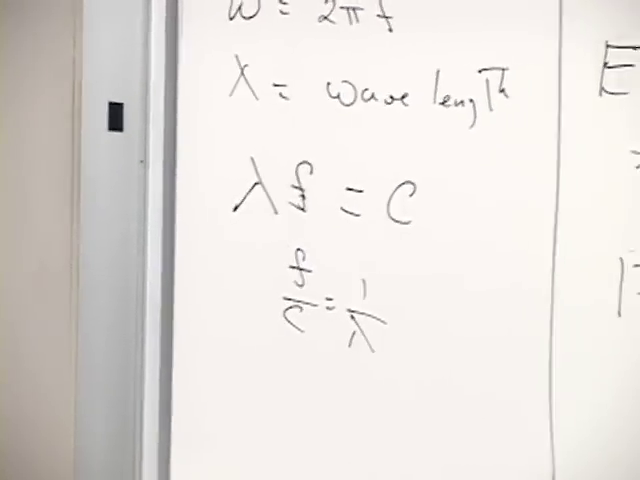
\includegraphics[width=0.56\textwidth]{lecture_02_figure_02.png}\caption{빛의 경우 \(\lambda f=c\)와 \(f/c=1/\lambda\)를 이용해 \(|\vec p_\gamma|=h/\lambda\)를 얻는다.}\lectureframe{00:21:39}\end{figure}

파장이 짧을수록 광자의 운동량은 커진다. 이것은 입자물리학에서 가장 중요한 양자적 사실 가운데 하나다. 작은 물체를 연구하려면 파장이 짧은 탐침이 필요하며, 파장을 짧게 하기 위해 치러야 하는 대가가 큰 운동량이다.

\begin{classroomqa}\lecturetimestamp{00:22:23}\audiencequestion{\(E=\hbar\omega\)은 근본적인가, 아니면 더 깊은 원리에서 유도되는가?}\lecturerresponse{조화진동자의 양자역학에서 나온다. 그 결과는 증명을 되풀이하지 않고 여기서 사용하겠다. 아래에서 다룰 진동자 표현을 통해 그 결과가 놓인 더 깊은 맥락을 살펴볼 수 있다.}\end{classroomqa}


\section{파동의 진폭과 광자 수}

\begin{classroomqa}\lecturetimestamp{00:23:10}\audiencequestion{광자의 관점에서 파동의 진폭은 무엇을 뜻하는가?}\lecturerresponse{진동수와 파장은 같지만 진폭은 다른 두 파동, 이를테면 \(\sin(kx)\)과 \(A\sin(kx)\)를 비교해 보자. 고전적으로 고정된 영역 안의 에너지는 진폭의 제곱에 비례한다. 양자역학적으로 \(n\)개의 광자를 포함한 모드의 에너지는 \(n\hbar\omega\)다. 따라서 진동수와 영역, 정규화를 고정하면 진폭의 크기는 대략 \(\sqrt n\)에 따라 커진다.}\end{classroomqa}

두 파동은 진동 양상이 같다. 한쪽이 단지 다른 쪽보다 더 강할 뿐이다.\footnote{도식은 00:23:47--00:24:28의 파동 비교를 따른다.}

\begin{figure}[t]\centering
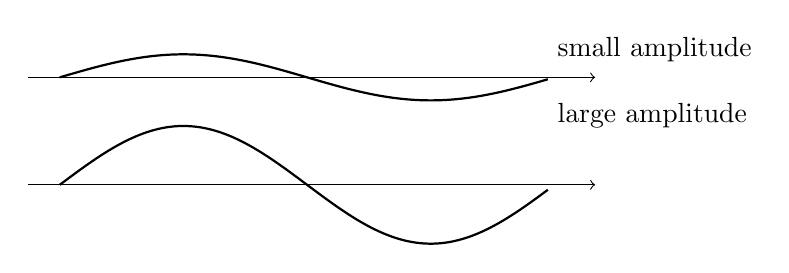
\begin{tikzpicture}[x=1cm,y=0.65cm]
\draw[->] (-0.4,0) -- (6.8,0);
\draw[->] (-0.4,-2.1) -- (6.8,-2.1);
\draw[thick] plot[domain=0:6.2,samples=120] (\x,{0.45*sin(\x r)});
\draw[thick] plot[domain=0:6.2,samples=120] (\x,{-2.1+1.15*sin(\x r)});
\draw (6.2,0.55) node[right]{small amplitude};
\draw (6.2,-0.75) node[right]{large amplitude};
\end{tikzpicture}\caption{파장과 진동수는 같고 진폭은 다른 파동.}\end{figure}

파동의 양을 고정하면, \begin{equation}
E_{\text{wave}}\propto A^2.
\end{equation}전자기파의 경우 이는 장의 에너지가 장의 세기 제곱에 비례한다는 익숙한 진술이다. 같은 모드에 \(n\)개의 광자가 들어 있다면, \begin{equation}
E_{\text{wave}}=n\hbar\omega.
\end{equation}따라서 모드와 진동수, 정규화, 영역을 고정했을 때, \begin{equation}
A^2\propto n\hbar\omega,
\qquad
A\propto\sqrt n\quad\text{at fixed }\omega.
\end{equation}정확한 정규화를 주장하는 것은 아니다. 포함된 파동의 양이 중요하다. 균일한 파동의 길이를 두 배로 하면 국소 진폭은 그대로지만 전체 에너지는 달라진다. 그러므로 이 비례 관계는 한 파장과 같은 고정된 영역에 대해 이해할 수 있다.

여기에는 양자역학 특유의 단서도 있다. 진폭과 위상에 동시에 고전적인 정확한 값을 지정할 수는 없다. 따라서 완벽하게 확정된 고전적 장을 묻는 것이라면 ``광자 하나의 진폭은 얼마인가?''라는 질문은 모호하다. 그럼에도 \(n=1\)로 두면 크기를 추정하는 합리적인 기준을 얻을 수 있다.

\begin{classroomqa}\lecturetimestamp{00:28:25}\audiencequestion{전자기파 그림에서 수직 변위는 공간 속 광자의 위치를 나타내는가?}\lecturerresponse{아니다. 전파축은 공간 방향이고, 수직 좌표는 전기장이나 자기장의 값을 나타낸다. 운동량은 전파축 방향을 향하며, 그래프에 표시된 장의 진폭 방향을 향하지 않는다.}\end{classroomqa}

파동은 어느 공간 방향으로든 전파될 수 있지만, 익숙한 사인파 그림에서는 수평축만 공간 좌표로 사용한다. 그래프의 다른 축은 장의 세기를 나타낸다.

\begin{classroomqa}\lecturetimestamp{00:29:37}\audiencequestion{파동의 광자 수는 파동의 한 파장이나 한 주기 안에 들어 있는 수를 세는 것인가?}\lecturerresponse{한 파장처럼 고정된 영역을 택할 수 있다. 비례 관계만 성립하는 이유가 여기에 있다. 전체 에너지와 광자 수도 파동에서 얼마나 많은 부분을 포함하느냐에 따라 달라진다. 진폭이 같아도 두 파장, 세 파장, 네 파장에 들어 있는 에너지는 한 파장에 들어 있는 에너지보다 그에 비례해 크다.}\end{classroomqa}

\begin{classroomqa}\lecturetimestamp{00:30:17}\audiencequestion{광자 하나의 진폭은 의미가 없는가?}\lecturerresponse{\(n=1\)로 두어 얻는 크기 추정으로만 의미가 있다. 전자기 모드에서 전기장과 자기장 정보는 서로 켤레인 위치와 운동량 정보에 유사한 역할을 하므로, 양자 불확정성이 고전적 진폭을 얼마나 정확히 지정할 수 있는지 제한한다. 그래도 크기 추정 관계는 유용하다.}\end{classroomqa}

이 질문들은 장 변수와 입자 수의 관계를 정확히 서술할 수 있는 양자장론으로 이어진다. 지금은 비례 관계만으로 충분하다.

\section{일반적인 양자 관계와 느린 물질파}

광자에 대해 도입한 몇몇 공식은 훨씬 더 일반적으로 적용되지만, 그렇지 않은 공식도 있다. 전자로 넘어가기 전에 이를 구분해 두자.

\begin{figure}[t]\centering
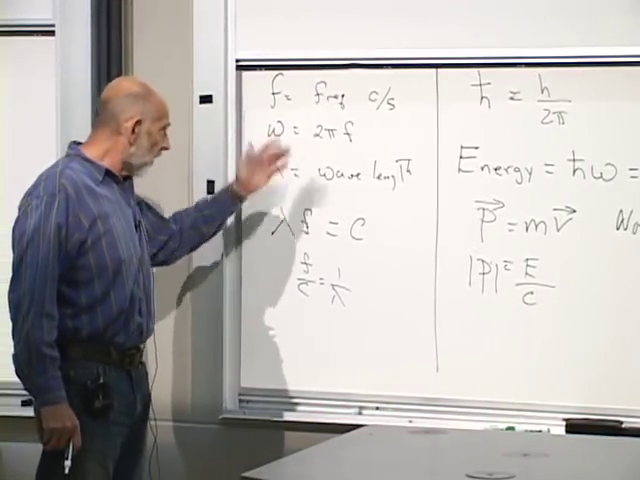
\includegraphics[width=0.82\textwidth]{lecture_02_figure_03.png}\caption{파동의 정의, 광자 운동량 관계와 비상대론적 운동량 관계의 적용 범위 비교.}\lectureframe{00:31:52}\end{figure}

\(f\), \(\omega=2\pi f\), \(\lambda\)의 정의는 일반적으로 적용된다. 이 논의에서 양자 관계 \begin{equation}
E=\hbar\omega=hf
\end{equation}도 일반적으로 성립한다. 반면 \(c\)가 포함된 공식, 예를 들어 \(\lambda f=c\)과 \(|\vec p|=E/c\)는 빛의 속력으로 움직이는 파동에 적용된다. 공식 \(\vec p=m\vec v\)은 빛보다 훨씬 느리게 움직이는 입자에 적용된다. 이 두 극한 사이의 상대론적 운동을 다루려면 보간 관계가 필요하지만, 아직은 필요하지 않다.

운동량--파장 관계는 광자의 예를 넘어 성립한다. \begin{equation}
p=\frac{h}{\lambda}.
\end{equation}여기서 \(p\)은 \(\lambda\)를 양의 파장으로 취했을 때 그 크기를 뜻한다. 방향은 따로 지정할 수 있다.

\begin{figure}[t]\centering
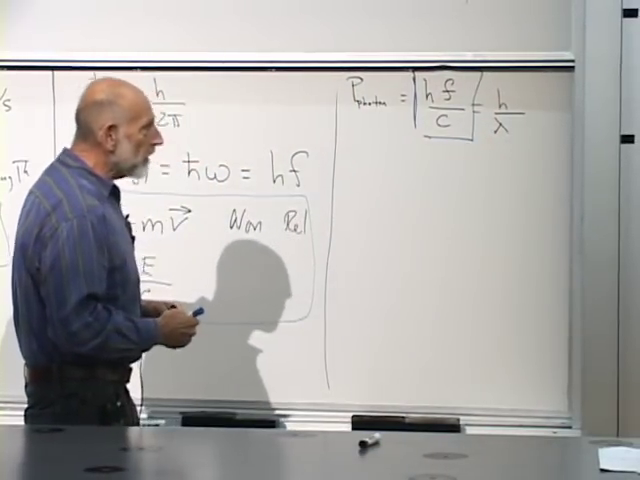
\includegraphics[width=0.74\textwidth]{lecture_02_figure_04.png}\caption{광자 운동량 \(|\vec p_\gamma|=hf/c=h/\lambda\)에서 일반적인 드브로이 관계로 이어진다.}\lectureframe{00:33:32}\end{figure}

전자, 원자핵은 물론이고 볼링공에도 파동을 대응시킬 수 있다. 전자 간섭은 그 사실이 드러나는 한 가지 사례다. 전자파를 \(\psi\)라 쓰자. 느리게 움직이는 전자에 대해서는 무엇이 \(\lambda f=c\)를 대신할까? 빠진 요소는 에너지와 운동량 사이의 비상대론적 관계다.

운동 에너지와 운동량에서 시작하자. \begin{align}
E&=\frac12 mv^2,\\
p&=mv,
\qquad
v=\frac{p}{m}.
\end{align}마지막 관계를 첫 번째 관계에 대입하면 \begin{align}
E
&=\frac12m\left(\frac{p}{m}\right)^2\\
&=\frac{p^2}{2m}.
\end{align}질량은 \(\frac12 mv^2\)에서는 분자에, \(p^2/(2m)\)에서는 분모에 놓인다. 이 위치는 혼동하기 쉬우므로 직접 다시 유도해 볼 만하다.

이제 일반적인 양자 관계를 쓰자. \begin{equation}
E=hf,
\qquad
p=\frac{h}{\lambda}.
\end{equation}느린 입자 하나에 대해서는, \begin{align}
hf
&=\frac{p^2}{2m}\\
&=\frac{1}{2m}\left(\frac{h}{\lambda}\right)^2\\
&=\frac{h^2}{2m\lambda^2}.
\end{align}\(h\)으로 나누면, \begin{equation}
f=\frac{h}{2m\lambda^2}.
\end{equation}

\begin{figure}[t]\centering
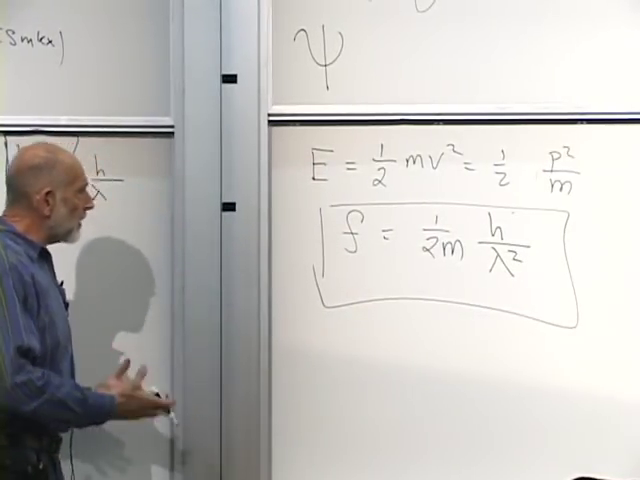
\includegraphics[width=0.64\textwidth]{lecture_02_figure_05.png}\caption{느린 입자에서는 \(E=p^2/(2m)\)과 \(p=h/\lambda\)로부터 \(f=h/(2m\lambda^2)\)을 얻는다.}\lectureframe{00:37:47}\end{figure}

빛의 경우, \begin{equation}
f\propto\frac{1}{\lambda},
\end{equation}인 반면 느린 물질의 경우, \begin{equation}
f\propto\frac{1}{\lambda^2}.
\end{equation}다. 두 번째 관계만 따로 외울 필요는 없다. \(E=p^2/(2m)\), \(E=hf\), \(p=h/\lambda\)에서 언제든 다시 유도할 수 있다. 원자 안에서 느리게 움직이는 전자에 적용하면, 이에 대응하는 Schr\"odinger 파의 진동수를 얻는다.

\begin{classroomqa}\lecturetimestamp{00:38:35}\audiencequestion{비상대론적 진동수--파장 관계는 전자 이외의 입자에도 적용되는가?}\lecturerresponse{그렇다. 빛보다 훨씬 느리게 움직이는 모든 입자에 적용된다. 느린 극한과 빛과 같은 극한 사이의 상대론적 보간은 별개의 주제다.}\end{classroomqa}

\begin{classroomqa}\lecturetimestamp{00:38:55}\audiencequestion{중성미자에는 어떤 관계를 적용해야 하는가?}\lecturerresponse{중성미자의 속력에 따라 다르다. 자연에서 만나는 중성미자의 대부분은 빛의 속력에 매우 가까운 속력으로 움직이므로 빛과 같은 극한의 관계가 좋은 근사다. 빛보다 훨씬 느리게 움직이는 중성미자라면 비상대론적 관계를 따라야 한다.}\end{classroomqa}

\editorialnote{중성미자 질문 직후에 오간 짧은 청중 문답은 진폭, 양자, 서로 다른 전자 파장을 다루지만, 발언이 심하게 손상되어 정확히 복원하기 어렵다. 복원 가능한 답변에서는 파장이 다른 경우의 진폭과 양자 사이의 일반 관계에 대한 논의를 뒤로 미룬다.}

\begin{classroomqa}\lecturetimestamp{00:39:56}\audiencequestion{가속기에서 나온 \(20\,\mathrm{keV}\) 전자는 느린가, 상대론적인가?}\lecturerresponse{느린 입자로 취급한다. \(c=1\)인 단위계에서는 질량, 에너지, 운동량을 같은 단위로 나타낼 수 있다. 전자의 정지 에너지 규모는 대략 \(0.5\,\mathrm{MeV}\)인 반면, \(20\,\mathrm{keV}\)는 이보다 훨씬 작다. 비상대론적 운동량 기준으로 쓰면 \(p\ll mc\)이다.}\end{classroomqa}

예제의 에너지 비교는 다음과 같다. \begin{equation}
K=20\,\mathrm{keV}\ll m_ec^2\simeq0.5\,\mathrm{MeV}.
\end{equation}\editorialnote{00:39:56--00:41:40의 원문 구절에서는 \(20\,\mathrm{keV}\)를 가속기 에너지로 제시한 다음, 상대론적 기준을 운동량과 정지 질량의 비교로 표현한다. 제시된 에너지를 운동량과 동일시하지 않으면서 비상대론적이라는 결론을 유지하려면 운동 에너지 기준과 운동량 기준을 따로 쓰면 된다.}

\section{위상 속도, 군속도와 분산}

\begin{classroomqa}\lecturetimestamp{00:41:46}\audiencequestion{진동수와 파장을 곱해 전자파의 속도를 구할 수 있는가?}\lecturerresponse{그렇게 얻는 것은 위상 속도이지 전자에 대응시키는 속도가 아니다. 국소화된 파동 묶음에는 내부 마루와 골의 운동을 나타내는 위상 속도와 포락선의 운동을 나타내는 군속도가 모두 있다. 군속도를 입자의 운동과 동일시한다.}\end{classroomqa}

파동 묶음은 국소적으로 사인파나 코사인파처럼 보이지만 포락선 안에 국한되어 있다. 파동 묶음이 움직일 때 포락선과 그 안의 마루가 같은 속력으로 움직일 필요는 없다.\footnote{도식은 00:42:34--00:44:11의 파동 묶음 논의를 따른다.}

\begin{figure}[t]\centering
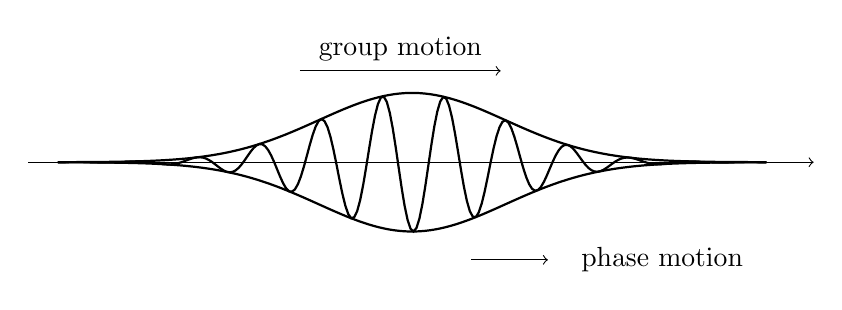
\begin{tikzpicture}[x=0.75cm,y=0.8cm]
\draw[->] (-0.5,0) -- (12.8,0);
\draw[thick] plot[domain=0:12,samples=140] (\x,{1.10*exp(-0.20*(\x-6)^2)});
\draw[thick] plot[domain=0:12,samples=140] (\x,{-1.10*exp(-0.20*(\x-6)^2)});
\draw[thick] plot[domain=0:12,samples=240] (\x,{1.10*exp(-0.20*(\x-6)^2)*sin(6*\x r)});
\draw[->] (4.1,1.45) -- (7.5,1.45);
\draw (5.8,1.8) node{group motion};
\draw[->] (7.0,-1.55) -- (8.3,-1.55);
\draw (8.7,-1.55) node[right]{phase motion};
\end{tikzpicture}\caption{포락선과 내부 위상이 일반적으로 서로 다른 속도로 움직이는 국소화된 파동 묶음.}\end{figure}

위상 속도는 단색 성분의 마루와 골, 그리고 다른 고정된 위상점들의 속도다. 비상대론적 분산 관계에서는, \begin{equation}
v_\phi=f\lambda=\frac{h}{2m\lambda}.
\end{equation}파장에 따라 달라진다. 따라서 파장이 다른 성분들은 위상 속도도 서로 다르고, 마루는 파동 묶음 안을 지나가며 파동 묶음은 분산될 수 있다. 군속도는 파동 묶음 전체의 속도이며, 입자의 속도와 동일시하는 값이다.

간단한 특수한 경우가 있다. 모든 파장 성분이 같은 속도로 움직이면 위상 속도와 군속도가 일치한다. 진공 속 빛은 이러한 성질을 갖는다. 모든 파장이 \(c\)의 속력으로 전파된다. 느린 입자에 대한 관계는 그렇지 않으며, 그 관계에서 \(f\lambda\)는 \(\lambda\)에 따라 달라진다.

방정식 \begin{equation}
f=\frac{h}{2m\lambda^2}
\end{equation}은 자유 Schr\"odinger 방정식을 조금 다른 형태로 쓴 것이다. 진동수는 평면파의 시간 의존성을, 파장은 공간 의존성을 정하며, Schr\"odinger 방정식은 두 의존성을 연결한다. 반대로, 진동수와 파장이 정해진 파동을 자유 Schr\"odinger 방정식에 대입해도 이 분산 관계를 얻는다.

\begin{classroomqa}\lecturetimestamp{00:47:02}\audiencequestion{위상 속도가 빛의 속력을 초과할 수 있는가?}\lecturerresponse{그렇다. 위상 속도는 정보를 전달하지 않는다. 정보와 국소화된 파동 묶음은 군속도로 전파되므로, 위상 속도가 광속보다 빠르더라도 광속보다 빠른 신호 전달이 가능해지는 것은 아니다.}\end{classroomqa}

\section{유한한 공간과 이산 운동량}

궁극적인 관심은 무한 공간의 파동에 있지만, 유한한 계에서 시작하는 편이 더 안전하다. 무한대는 컴퓨터가 직접 저장하거나 조작할 수 있는 것이 아니다. 먼저 유한한 계에 대한 방정식을 세우고 나서, 계의 크기를 한없이 크게 만드는 극한을 취한다. 이 습관은 양자역학, 양자장론, 입자물리학 전반에서 유용하다.

한 공간 차원에서 시작해도 본질적인 것을 잃지 않는다. 파동은 바이올린 줄이나 흔들리는 밧줄 위에 있을 수도 있고, 추상적인 1차원 세계에 있을 수도 있다. 가장 명백한 유한계는 길이 \(L\)인 선분과 그 양 끝의 반사 경계다. 파동은 한쪽 끝까지 가서 반사된 뒤 되돌아온다. 이는 완전히 타당한 반사 경계 조건이지만 한 가지 불편함이 있다. 파동계 안에서 운동량이 보존되지 않는다. 오른쪽으로 진행하는 파동은 오른쪽 방향의 운동량을 가진다. 반사된 뒤에는 왼쪽 방향의 운동량을 가진다. 경계가 충격량을 가하고 그 차이를 흡수한 것이다.

반사 경계에서 운동량이 뒤집히는 모습을 도식으로 나타낼 수 있다.\footnote{도식은 00:49:24--00:51:08의 반사 경계 논의를 따른다.}

\begin{figure}[t]\centering
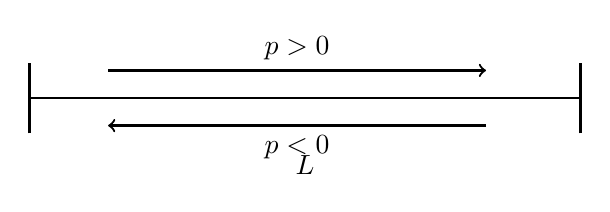
\begin{tikzpicture}[x=1cm,y=1cm]
\draw[thick] (0,0) -- (7,0);
\draw[very thick] (0,-0.45) -- (0,0.45);
\draw[very thick] (7,-0.45) -- (7,0.45);
\draw[->,thick] (1.0,0.35) -- (5.8,0.35) node[midway,above]{\(p>0\)};
\draw[->,thick] (5.8,-0.35) -- (1.0,-0.35) node[midway,below]{\(p<0\)};
\draw (3.5,-0.85) node{\(L\)};
\end{tikzpicture}\caption{유한한 선분의 양 끝에서 반사되면 진행하는 파동의 운동량이 반전된다.}\end{figure}

운동량을 보존하면서 계를 유한하게 만드는 다른 방법이 있다. 선분의 두 끝점을 서로 동일시하는 것이다. 그 결과를 원으로 그릴 수는 있지만, 2차원 공간 안에 실제 원이 놓여 있어야 하는 것은 아니다. 수학적으로는 좌표가 주기적이라는 뜻이다. 총 거리 \(L\)만큼 이동한 뒤에는 같은 점으로 돌아온다.

\begin{figure}[t]\centering
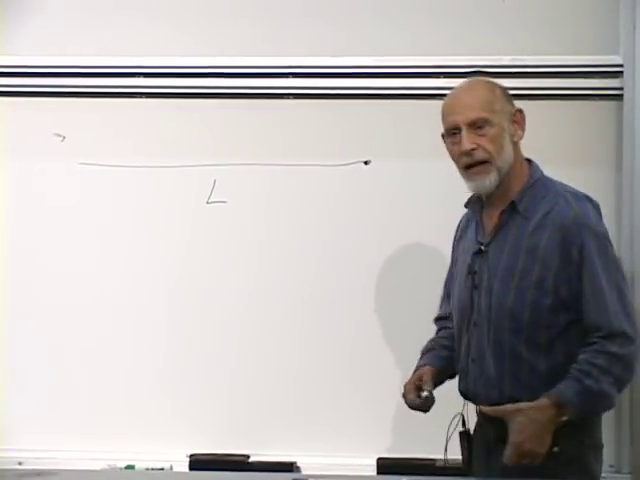
\includegraphics[width=0.72\textwidth]{lecture_02_figure_06.png}\caption{길이 \(L\)인 경로를 주기적으로 동일시하는 방법을 소개한다.}\lectureframe{00:51:21}\end{figure}

다음 도식에서 끝점의 동일시를 명시적으로 나타낸다.\footnote{도식은 00:51:09--00:52:37의 주기적 동일시 논의를 따른다.}

\begin{figure}[t]\centering
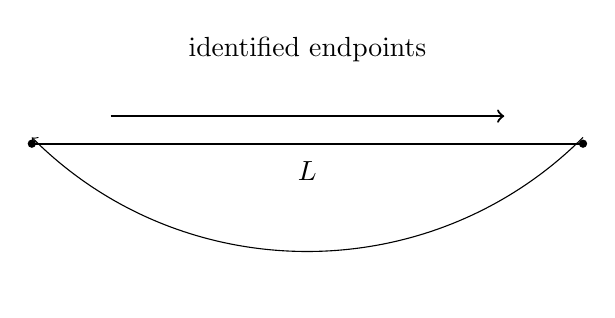
\begin{tikzpicture}[x=1cm,y=1cm]
\draw[thick] (0,0) -- (7,0);
\fill (0,0) circle (1.5pt);
\fill (7,0) circle (1.5pt);
\draw[->,thick] (1.0,0.35) -- (6.0,0.35);
\draw (3.5,-0.35) node{\(L\)};
\draw[->,bend left=45] (7,0.08) to (0,0.08);
\draw (3.5,1.2) node{identified endpoints};
\end{tikzpicture}\caption{길이 \(L\)인 경로의 양 끝점을 동일시해 만든 주기적인 1차원 공간.}\end{figure}

그러면 오른쪽으로 가는 파동은 그림에 표시된 끝점에 도달한 뒤 처음으로 다시 나타나 계속 오른쪽으로 진행한다. 왼쪽으로 가는 파동도 계속 왼쪽으로 진행한다. 파동이 반사되는 특별한 끝점이 없으므로 운동량은 반전되지 않는다. 주기적 공간은 부피를 유한하게 유지하면서 운동량을 보존하지만, 중요한 결과가 따른다. 허용되는 운동량이 이산적이다.

정수 개의 파장이 전체 길이에 들어맞아야 한다. 상수가 아닌 모드의 경우, \begin{equation}
\lambda_{|N|}=\frac{L}{|N|},
\qquad |N|=1,2,3,\ldots .
\end{equation}따라서 파장의 크기는 \(L\), \(L/2\), \(L/3\) 등일 수 있다. \(L/\sqrt{2}\)와 같은 선택은 들어맞지 않는다. 한 바퀴 돈 뒤 파동이 위상이 맞지 않는 채 돌아와 시작점의 값과 일치하지 않기 때문이다.

\(p=h/\lambda\)을 이용하면 \(|N|\)번째 비상수 모드의 운동량 크기는
\begin{equation}
|p_N|=\frac{|N|h}{L}.
\end{equation}
양방향과 상수 모드를 모호함 없이 모두 포함하려면 모드 표지를 부호 있는 값으로 두는 것이 편리하다:
\begin{equation}
p_N=\frac{Nh}{L},
\qquad N=0,\pm1,\pm2,\ldots .
\end{equation}
\(N\)의 양수와 음수는 서로 반대 방향의 전파를 나타낸다. \(N=0\) 모드는 상수이고 운동량이 0이며, \(h/\lambda\)에 대입할 유한한 파장은 없다. 따라서 기본 운동량 간격은 \(h/L\)이다.

거시적인 \(L\)에서는 \(h\)와 \(1/L\) 모두 이 간격을 극도로 작게 만들므로, 허용값들은 매우 빽빽하게 분포해 거의 연속적으로 보인다. 그래도 원형 도선에 구속된 구슬의 스펙트럼은 정확히 이산적이다.

\begin{classroomqa}\lecturetimestamp{00:58:27}\audiencequestion{양자화되는 것은 파동의 전체 운동량인가, 아니면 한 주기에 해당하는 운동량인가?}\lecturerresponse{이 진술은 양자 하나의 운동량에 적용된다. 양자마다 허용된 이산 운동량 가운데 하나를 갖는다. 따라서 여러 양자가 모인 계의 전체 운동량도 기본 단위 \(h/L\)의 정수배가 된다.}\end{classroomqa}

\begin{classroomqa}\lecturetimestamp{00:59:22}\audiencequestion{파동은 왜 한 바퀴 돈 뒤 같은 값으로 돌아와야 하는가?}\lecturerresponse{동일시된 끝점은 같은 물리적 점이므로, 관측 가능한 장은 그곳에서 같은 값을 가져야 한다. 값이 맞지 않으면 그 점에서 장이 갑자기 불연속적으로 뛰어야 한다. 그런 불연속에는 에너지와 운동량이 많이 들기 때문에, 허용되는 장의 배치는 연속적이고 주기적이다.}\end{classroomqa}

\begin{classroomqa}\lecturetimestamp{01:00:09}\audiencequestion{파동이 파동 묶음으로 국소화되면 어떻게 되는가?}\lecturerresponse{파동 묶음은 평면파, 또는 사인과 코사인의 푸리에 합이다. 주기적 공간에서 그 합에는 허용된 이산 운동량 모드만 포함될 수 있다. 따라서 양자화에 관한 진술은 허용되는 모든 파동 묶음의 푸리에 성분에 관한 진술이다.}\end{classroomqa}

\begin{classroomqa}\lecturetimestamp{01:01:01}\audiencequestion{주기 길이 \(L\)가 극도로 작아지면 문제가 생기는가?}\lecturerresponse{\(L\)가 작아질수록 기본 운동량 \(h/L\)은 매우 커진다. 보통의 미시적 길이에서는 당장 모순이 생긴다는 뜻은 아니지만, 이 구성을 플랑크 길이 규모까지 밀어붙이려면 새로운 물리학이 필요할 것으로 예상된다.}\end{classroomqa}

이제 원형 그림을 문자 그대로 받아들여 보자. 반지름이 \(r\)인 원형 도선 위에서 구슬이 움직이며, 원주의 길이는 \(L=2\pi r\)이다. 허용되는 접선 방향 운동량은 \begin{equation}
p_N=\frac{Nh}{2\pi r}=\frac{N\hbar}{r}.
\end{equation}이다. 원형 궤도를 도는 비상대론적 입자의 각운동량은 \(mvr\)이다. 이 영역에서 \(p=mv\)이므로 이는 \(rp\)이다. \(mvr\)라는 표현은 상대론적으로 일반적인 관계가 아니다. 상대론적 영역에서는 \(p\)가 단순히 \(mv\)와 같지 않기 때문이다. 하지만 운동량과 수직 거리의 곱은 여전히 올바른 관계다. 벡터로 쓰면,\footnote{강의에서는 먼저 각운동량에 \(L\)을 사용했다가, 주기적 길이를 나타내는 \(L\)와 기호가 겹친다는 점을 알아채고 기호를 바꾼다. 여기서는 전체에 걸쳐 \(J\)를 사용한다. 01:03:40--01:05:21을 참조하라.}\begin{equation}
\vec J=\vec r\times\vec p,
\end{equation}접선 방향 원운동에서는 그 크기가 \(J=rp\)이다. 그러므로 \begin{equation}
J_N=rp_N=N\hbar.
\end{equation}선운동량 간격은 원의 크기에 따라 달라지지만, 각운동량의 단위는 언제나 \(\hbar\)이다. 페르미온이 관여하면 정수 규칙에 예외가 생기는데, 그 예외는 뒤에서 다룬다.

다음 과제는 장과 입자, 양자를 더 정확히 연결하는 것이다. 그러려면 연산자와 조화진동자의 양자역학으로 잠시 돌아가야 한다.

\section{파동 모드와 양자 연산자}

이어지는 양자역학은 필연적으로 추상적이며 복습을 위한 것이다. 파동은 진동이므로 조화진동자가 핵심적인 계다. 고정된 한 점에서 전기장이나 자기장, 또는 다른 파동 진폭은 시간에 따라 주기적으로 변한다. 성분의 진동수가 있다고 말하는 것은 곧 그 성분이 진동한다고 말하는 것이다.

일반적인 파동이 반드시 하나의 파장만을 갖는 것은 아니다. 여러 색의 빛을 섞을 수 있고, 반대로 뉴턴이 백색광을 분해했을 때처럼 프리즘으로 혼합광을 구성 색으로 나눌 수도 있다. 각 성분은 고유한 파장, 진동수, 진폭, 에너지, 운동량을 갖는다. 따라서 혼합된 파동은 에너지와 운동량이 서로 다른 양자로 분해할 수 있다. 각 파장은 하나의 진동수를 정하고, 진동수가 정해진 각 성분은 진동자처럼 거동한다. 그러므로 임의의 양자계가 아니라 조화 진동자가 장의 자연스러운 기본 구성 요소가 된다.

양자 관측량은 연산자로 나타낸다. 연산자는 더하고 곱할 수 있지만, 보통의 수와 달리 곱의 순서에 따라 결과가 달라질 수 있다. \(A\)와 \(B\)를 각각 계의 두 성질을 나타내는 연산자라고 하자. 각 성질은 따로 측정할 수 있을지도 모른다. 예를 들어 \(A\)는 전기장을, \(B\)는 자기장을 나타낼 수 있다. 측정값이 보통의 수 \(a\)와 \(b\)라면 \begin{equation}
ab=ba.
\end{equation} 수치의 곱은 곱셈 순서에 따라 달라질 수 없다. 그러나 양자역학에서는 이에 대응하는 연산자들이 대신 \(AB-BA\neq0\)을 만족할 수 있다.

처음에는 이것이 말이 안 되는 것처럼 보인다. 전기장을 측정하면 하나의 수가 나오고 자기장을 측정하면 또 다른 수가 나온다면, 그 두 수를 곱한 결과는 어느 순서로 곱하든 같아야 한다. 해답은 연산자 곱이 순서에 따라 달라질 때 두 물리량을 동시에 측정할 수 없다는 것이다. 한쪽을 측정하는 실험이 다른 쪽의 측정을 방해한다. 두 수치값을 함께 얻을 수 없으므로 모순은 없다.

두 물리량을 동시에 측정할 수 있다면, 측정값은 보통의 수이며 이 수들은 서로 가환한다. 따라서 동시 측정 가능성을 판별하는 기준은 교환자이다.
\begin{equation}
[A,B]=AB-BA.
\end{equation}
교환자가 영이면 관측량은 양립 가능하고, 영이 아니면 해당 측정들은 서로 간섭한다. 항의 순서를 뒤바꾸면 부호가 바뀐다:
\begin{equation}
[B,A]=-[A,B].
\end{equation}

비상대론적 입자에서는 위치의 세 성분이 서로 가환하며, 운동량의 세 성분도 서로 가환한다:
\begin{align}
[x,y]&=[y,z]=[z,x]=0,\\
[p_x,p_y]&=[p_y,p_z]=[p_z,p_x]=0.
\end{align}
세 좌표를 모두 함께 정할 수 있고, 운동량의 세 성분도 모두 함께 정할 수 있다. 서로 대응하는 위치 성분과 운동량 성분은 가환하지 않는다:
\begin{equation}
[x,p_x]=[y,p_y]=[z,p_z]=i\hbar,
\end{equation}
반면 \([x,p_y]\)와 같은 혼합 성분의 교환자는 영이다. 위치 좌표를 측정하면 입자에 켤레 운동량의 교란이 생긴다. 다시 말해, 대응하는 위치와 운동량의 불확정성 곱은 \(\hbar\)에 의해 제한된다.

\begin{classroomqa}\lecturetimestamp{01:16:30}\audiencequestion{\(x\)에서 \(y\)로 바꿀 때, 교환자 안의 \(i\)를 \(j\)로 바꾸어야 하나요?}\lecturerresponse{아니요. 기호 \(i\)는 항상 허수 단위, 즉 마이너스 1의 제곱근입니다. 데카르트 단위벡터의 첨자도 아니고, 사원수 기호 \(i,j,k\) 중 하나도 아닙니다.}\end{classroomqa}

\begin{classroomqa}\lecturetimestamp{01:17:24}\audiencequestion{\(AB-BA\)은 먼저 \(A\)를 측정하고 그다음 \(B\)를 측정한 뒤, 측정 순서를 뒤집는다는 뜻인가요?}\lecturerresponse{아니요. 두 항은 연산자 또는 행렬을 서로 다른 대수적 순서로 곱한 것입니다. 실제 측정을 차례로 한다는 뜻이 아닙니다. 양립할 수 없는 측정과의 연관성은 연산자 대수에서 따라 나오는 결과이지, 곱의 정의가 아닙니다.}\end{classroomqa}

\begin{classroomqa}\lecturetimestamp{01:18:32}\audiencequestion{이 위치--운동량 교환자는 광자에도 직접 적용되나요?}\lecturerresponse{직접 적용되지는 않습니다. 이 관계는 비상대론적 입자에 깔끔하게 적용됩니다. 광자의 위치는 정의하기가 더 까다로우므로 유사한 설명에는 더 세심한 주의가 필요하며, 여기서는 다루지 않아도 됩니다.}\end{classroomqa}

\section{양자 조화 진동자}

스프링에 매달린 추, 음파, 광파는 모두 진동 운동의 예다. 모든 이상적인 조화 진동자는 진동수를 갖는다. 스프링의 경우 한 주기는 추가 같은 위치로 돌아오는 데 걸리는 시간만을 뜻하지 않는다. 같은 방향으로 움직이면서 그 위치로 돌아와야 한다. 초당 완전한 주기의 수를 \(f\)라 하고, \(\omega=2\pi f\)이다.

고전적으로 이상적인 진동자는 음이 아닌 임의의 에너지를 가질 수 있다. 살짝 밀면 에너지가 작고, 더 세게 밀면 에너지가 커진다. 실제 스프링은 결국 부러지거나 녹겠지만, 수학적 이상화에서는 양의 에너지가 연속적으로 분포한다. 양자 진동자는 다르다. 허용된 에너지는 서로 같은 간격으로 떨어진 이산적인 준위를 이룬다. 에너지의 기준점을 정해 가장 낮은 준위를 0이라 하면 \begin{equation}
E_n=n\hbar\omega,
\qquad n=0,1,2,\ldots .
\end{equation} 같은 간격의 준위는 다음과 같이 그려 볼 수 있다.\footnote{에너지 준위 개략도는 판서 설명 01:21:20--01:23:56을 따른다.}

\begin{figure}[t]\centering
\begin{tikzpicture}[x=1cm,y=0.9cm]
\draw[->] (0,0) -- (0,5.35);
\draw (0,5.5) node[above]{energy};
\foreach \y/\lab in {0.6/{0},1.6/{\hbar\omega},2.6/{2\hbar\omega},3.6/{3\hbar\omega},4.6/{n\hbar\omega}}
{
  \draw[thick] (0.2,\y) -- (2.2,\y);
  \draw (-0.25,\y) node[left]{\(\lab\)};
}
\draw[->,thick] (2.8,0.68) -- (2.8,1.52);
\draw (3.2,1.1) node[right]{\(a_+\)};
\draw[->,thick] (3.7,1.52) -- (3.7,0.68);
\draw (4.1,1.1) node[right]{\(a_-\)};
\end{tikzpicture}\caption{규약 \(E_n=n\hbar\omega\)에 따른 등간격 진동자 준위.}\end{figure}

준위 간격 \(\hbar\omega\)은 앞서 각진동수 \(\omega\)인 광자 하나에 부여한 에너지와 같다. \(2\hbar\omega\)은 진동수 \(2\omega\)인 진동자의 양자 하나의 에너지일 수도 있고, 진동수 \(\omega\)인 진동자에 든 양자 두 개의 에너지일 수도 있다. 여기서 필요한 해석은 두 번째다. 진동수가 고정된 하나의 진동자에는 양자가 0개, 1개, 2개, 3개 또는 그 이상 들어갈 수 있으며, 준위 사이에 허용되는 에너지는 없다.

정수 \(n\)는 진동자 상태를 나타내며, 상태는 켓 \(|n\rangle\)로 쓴다. \(|0\rangle\)는 바닥 상태이고, \(|1\rangle\)에는 들뜸 양자가 하나, \(|2\rangle\)에는 두 개 있으며, 이런 식으로 이어진다. 켓은 연산자가 작용하는 상태를 나타내는 표기일 뿐이다.

상태를 한 준위 올리는 상승 연산자 \(a_+\)와 한 준위 내리는 하강 연산자 \(a_-\)를 정의하자. \begin{align}
a_+|n\rangle &= \sqrt{n+1}\,|n+1\rangle,\\
a_-|n\rangle &= \sqrt{n}\,|n-1\rangle.
\end{align} 최저 상태에서는 \begin{equation}
a_-|0\rangle=0,
\end{equation} 바닥 상태보다 낮은 상태가 없기 때문이다.

여기서는 보통의 수와 연산자를 구별하는 것이 중요하다. 표지 \(n\)와 \(\sqrt n\) 같은 계수는 보통의 수이므로 모든 것과 교환한다. 기호 \(a_+\)와 \(a_-\)는 연산자이므로 순서를 유지해야 한다.

먼저 \(|n\rangle\)를 낮춘 다음 다시 올려 보자. 내리는 단계는 다음과 같다. \begin{equation}
a_-|n\rangle=\sqrt n\,|n-1\rangle.
\end{equation} 그 결과로 얻은 상태에 \(a_+\)를 작용시키면 계수 \(\sqrt n\)가 다시 붙는다. \(|n-1\rangle\)를 올리면 \(|n\rangle\)로 돌아오기 때문이다. \begin{align}
a_+a_-|n\rangle
&=a_+\bigl(\sqrt n\,|n-1\rangle\bigr)\\
&=\sqrt n\,\sqrt n\,|n\rangle\\
&=n|n\rangle.
\end{align} 따라서 \(a_+a_-\)는 준위 번호를 읽어 낸다. 예를 들어 \(|\chi\rangle\)가 수 연산자의 고유상태라는 것은 알지만 준위 표지는 모른다고 하자. \begin{equation}
a_+a_-|\chi\rangle=q|\chi\rangle,
\end{equation}라면 보통의 수치 계수 \(q\)가 그 상태에 있는 양자의 수다. 따라서 이 곱이 수 연산자다. \begin{equation}
\hat n=a_+a_-,
\end{equation} 그리고 선택한 에너지 규약에서 해밀토니안은 다음과 같다. \begin{equation}
H=\hbar\omega\,a_+a_-.
\end{equation} 실제로 어느 준위에 작용시켜도 \(H|n\rangle=n\hbar\omega|n\rangle\)가 된다.

이제 순서를 바꾸어 보자. 먼저 올리면 \(\sqrt{n+1}|n+1\rangle\)가 된다. 이어서 내리면 \(|n\rangle\)로 돌아오고 계수 \(\sqrt{n+1}\)가 한 번 더 붙는다. \begin{align}
a_-a_+|n\rangle
&=a_-\bigl(\sqrt{n+1}\,|n+1\rangle\bigr)\\
&=\sqrt{n+1}\,\sqrt{n+1}\,|n\rangle\\
&=(n+1)|n\rangle.
\end{align} 두 순서는 모든 상태에서 1만큼 차이가 나므로 \begin{equation}
[a_-,a_+]=a_-a_+-a_+a_-=1.
\end{equation}

진동자에는 진폭과 위상도 있다. 위상은 진동 주기에서 현재 어느 지점에 있는지를 나타낸다. 구체적으로는 진동자가 정해 둔 방향으로 원점을 통과하는 시각으로 위상을 정할 수 있다. 그 통과 시각을 늦추면 진동수는 바뀌지 않고 위상만 달라진다. 사다리 연산자는 진폭과 위상에 해당하는 양자 변수들을 결합한다. 그 대수는 본질적으로 양자적이지만 작용은 간단하다. \(a_+\)는 진동자 에너지 양자를 하나 더하고, \(a_-\)는 하나 제거한다. 전자기 모드에서는 그 양자가 광자이므로 두 연산자를 각각 생성 연산자와 소멸 연산자라고 부른다.

\begin{classroomqa}\lecturetimestamp{01:37:34}\audiencequestion{상승 연산자와 하강 연산자는 물리적 측정에 대응하나요?}\lecturerresponse{광자 수는 측정할 수 있습니다. 추가적인 기술적 이유 때문에 연산자 \(a_+\)와 \(a_-\)는 각각 따로 측정 가능한 관측량이 아닙니다. 이들의 교환자는 둘이 교환하지 않음을 보여 주지만, 그 사실만으로 어느 한 연산자가 개별적으로 관측 불가능하다고 주장하는 것은 아닙니다.}\end{classroomqa}

자연 진동수가 서로 다른 스프링들을 모으면 독립 진동자들이 여럿 생긴다. 공동의 전자기 모드들도 마찬가지다. 다른 모드들도 같은 만큼 들떠 있어야 하는 것은 아니며, 한 파장만 들뜰 수 있다. 양자역학에서는 각 독립 진동자에서 생성 및 소멸 연산자가 고정된 진동수의 양자를 넣고 뺀다. 입자는 바로 그런 양자로 정의되므로 이 표현 방식은 핵심적이다.

\section{진동자들의 집합으로 본 장}

전체 길이가 \(L\)인 주기적 1차원 공간으로 돌아가자. 상수 모드가 아닌 모드들의 파장 크기는 \begin{equation}
\lambda_N=\frac{L}{N},
\qquad N=1,2,3,\ldots ,
\end{equation}이고, 이에 대응하는 음이 아닌 각진동수는 \(\omega_N\)이다. 앞서 다룬 운동량 스펙트럼과 비교하기 쉽도록, 부호가 있는 정수의 표지를 \(M\)로 다시 쓰자. \begin{equation}
p_M=\frac{Mh}{L},
\qquad M=0,\pm1,\pm2,\ldots .
\end{equation} \(M\)의 부호는 전파 방향을 나타낸다. \editorialnote{01:42:08--01:42:24에서 진동수 모드의 첨자 범위를 부호가 있는 정수에서 0부터 시작하는 범위로 바로잡았다. 기호 \(M\)는 부호가 있는 운동량 표기와 음이 아닌 진동수 모드 표지 \(N\)를 구분하기 위해서만 쓴다. 이는 \(+M\)와 \(-M\)에 독립적인 점유수를 도입하는 것이 아니다. 상수가 아닌 진동자 목록은 \(N=1\)에서 시작한다.}

허용된 각 진동수는 조화 진동자처럼 거동한다. 한 진동수에 에너지를 더한 다음 다른 진동수에 독립적으로 에너지를 더할 수 있다. 양자장의 자세한 첫 번째 예는 다음 강의로 미루지만, 상태 표기는 이미 분명하다. 상수가 아닌 모드들을 파장이 긴 순서로 나열하여 다음과 같이 쓰자. \begin{equation}
|n_1,n_2,n_3,\ldots\rangle,
\end{equation} 여기서 \(n_N=0,1,2,\ldots\)는 진동수 \(\omega_N\)인 진동자에 든 양자의 수다. 첫째 항목은 파장이 가장 긴 모드에 든 양자의 수를, 둘째 항목은 그다음 모드에 든 양자의 수를 나타내며, 이런 식으로 끝없이 이어진다.

현의 고조파를 보면 이 구성을 구체적으로 이해할 수 있다. 기본 진동에서 그다음 두 고조파까지의 진행을 개략적으로 보였다.\footnote{개략도는 현의 고조파에 관한 설명 01:45:20--01:47:46을 따른다.}

\begin{figure}[t]\centering
\resizebox{\linewidth}{!}{%
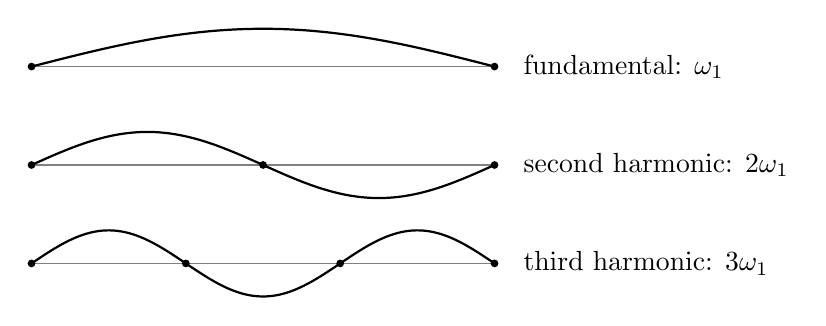
\begin{tikzpicture}[x=0.98cm,y=1cm]
\draw[gray] (0,2.5) -- (6,2.5);
\draw[thick] plot[domain=0:6,samples=120] (\x,{2.5+0.48*sin(30*\x)});
\fill (0,2.5) circle (1.4pt);
\fill (6,2.5) circle (1.4pt);
\node[right] at (6.25,2.5) {fundamental: \(\omega_1\)};

\draw[gray] (0,1.25) -- (6,1.25);
\draw[thick] plot[domain=0:6,samples=120] (\x,{1.25+0.42*sin(60*\x)});
\fill (0,1.25) circle (1.4pt);
\fill (3,1.25) circle (1.4pt);
\fill (6,1.25) circle (1.4pt);
\node[right] at (6.25,1.25) {second harmonic: \(2\omega_1\)};

\draw[gray] (0,0) -- (6,0);
\draw[thick] plot[domain=0:6,samples=120] (\x,{0.42*sin(90*\x)});
\fill (0,0) circle (1.4pt);
\fill (2,0) circle (1.4pt);
\fill (4,0) circle (1.4pt);
\fill (6,0) circle (1.4pt);
\node[right] at (6.25,0) {third harmonic: \(3\omega_1\)};
\end{tikzpicture}%
}\caption{현의 기본 진동과 두 번째 및 세 번째 고조파. 각각 마디가 내부에 0개, 1개, 2개 있다.}\end{figure}

기본 진동은 넓은 아치 하나처럼 움직이며 내부 마디가 없다. 하나의 진동자이므로 \(n_1=0,1,2,\ldots\)개의 양자를 가질 수 있고, 들뜸마다 \(\hbar\omega_1\)의 에너지가 든다. 두 번째 고조파에는 내부 마디가 하나 있으며 진동수는 두 배다. 기본 진동이 가온다라면 이 모드는 한 옥타브 높은 가온다로 들린다. 이 모드는 독립적인 점유수 \(n_2\)를 가지며, 양자 하나의 에너지는 \(\hbar\omega_2=2\hbar\omega_1\)이다. 세 번째 고조파에는 내부 마디가 두 개 있으며 진동수는 기본 진동의 세 배다. 이 모드는 독립적인 점유수 \(n_3\)를 가지며, 이 역시 음이 아닌 임의의 정수일 수 있다.

위에서 사용한 에너지 관례에 따르면, 각 모드에서 에너지는 점유수와 양자 에너지의 곱이다. 이 기여들을 모두 합하면 다음과 같다.
\begin{equation}
E=\sum_{N=1}^{\infty} n_N\hbar\omega_N.
\end{equation}
\editorialnote{이 표시된 합은 각 모드의 에너지를 따로 제시한 내용을 대수적으로 모아 쓴 것이다. 그 내용은 다음 위치에 제시되어 있다: 01:44:02--01:47:46.}

각 장 모드마다 같은 조화 진동자 수학을 적용해야 하므로, 독립 진동자 하나마다 생성 연산자 하나와 소멸 연산자 하나가 필요하다. 이 기초적인 그림에서 양자장은 진동자 전체와 그 생성--소멸 대수로 이루어진다.

이 표현 방식은 입자 산란에 맞춰져 있다. 에너지와 운동량이 정해진 양자들이 실험에 들어가고, 다른 에너지와 운동량을 가진 양자들이 나온다. 소멸 연산자가 초기 입자를 제거하고, 해당 모드의 생성 연산자가 최종 상태에 나가는 입자를 넣는다.

\begin{classroomqa}\lecturetimestamp{01:49:38}\audiencequestion{진동자 모드를 표시하는 정수와 그 안의 양자 수를 세는 정수가 같은 것인가요?}\lecturerresponse{서로 다른 정수가 두 개 있습니다. 모드 표지 \(N\)는 공간적 형태를 나타냅니다. 현의 예에서는 마디 수가 진동수 \(\omega_N\)를 정합니다. 점유수 \(n_N\)는 그 진동수를 가진 양자가 몇 개 있는지 나타냅니다.}\end{classroomqa}